\documentclass[journal,12pt,twocolumn]{IEEEtran}

\usepackage{setspace}
\usepackage{gensymb}
\singlespacing
\usepackage[cmex10]{amsmath}
\usepackage{amssymb}
\usepackage{xurl}

\usepackage{amsthm}
\usepackage{comment}
\usepackage{mathrsfs}
\usepackage{txfonts}
\usepackage{stfloats}
\usepackage{bm}
\usepackage{cite}
\usepackage{cases}
\usepackage{subfig}

\usepackage{longtable}
\usepackage{multirow}

\usepackage{enumitem}
\usepackage{mathtools}
\usepackage{steinmetz}
\usepackage{tikz}
\usepackage{circuitikz}
\usepackage{verbatim}
\usepackage{tfrupee}
\usepackage[breaklinks=true]{hyperref}
\usepackage{graphicx}
\usepackage{tkz-euclide}

\usetikzlibrary{calc,math}
\usepackage{listings}
    \usepackage{color}                                            %%
    \usepackage{array}                                            %%
    \usepackage{longtable}                                        %%
    \usepackage{calc}                                             %%
    \usepackage{multirow}                                         %%
    \usepackage{hhline}                                           %%
    \usepackage{ifthen}                                           %%
    \usepackage{lscape}     
\usepackage{multicol}
\usepackage{chngcntr}

\DeclareMathOperator*{\Res}{Res}

\renewcommand\thesection{\arabic{section}}
\renewcommand\thesubsection{\thesection.\arabic{subsection}}
\renewcommand\thesubsubsection{\thesubsection.\arabic{subsubsection}}

\renewcommand\thesectiondis{\arabic{section}}
\renewcommand\thesubsectiondis{\thesectiondis.\arabic{subsection}}
\renewcommand\thesubsubsectiondis{\thesubsectiondis.\arabic{subsubsection}}


\hyphenation{op-tical net-works semi-conduc-tor}
\def\inputGnumericTable{}                                 %%

\lstset{
%language=C,
frame=single, 
breaklines=true,
columns=fullflexible
}
\begin{document}


\newtheorem{theorem}{Theorem}[section]
\newtheorem{problem}{Problem}
\newtheorem{proposition}{Proposition}[section]
\newtheorem{lemma}{Lemma}[section]
\newtheorem{corollary}[theorem]{Corollary}
\newtheorem{example}{Example}[section]
\newtheorem{definition}[problem]{Definition}

\newcommand{\BEQA}{\begin{eqnarray}}
\newcommand{\EEQA}{\end{eqnarray}}
\newcommand{\define}{\stackrel{\triangle}{=}}
\bibliographystyle{IEEEtran}
\raggedbottom
\setlength{\parindent}{0pt}
\providecommand{\mbf}{\mathbf}
\providecommand{\pr}[1]{\ensuremath{\Pr\left(#1\right)}}
\providecommand{\qfunc}[1]{\ensuremath{Q\left(#1\right)}}
\providecommand{\sbrak}[1]{\ensuremath{{}\left[#1\right]}}
\providecommand{\lsbrak}[1]{\ensuremath{{}\left[#1\right.}}
\providecommand{\rsbrak}[1]{\ensuremath{{}\left.#1\right]}}
\providecommand{\brak}[1]{\ensuremath{\left(#1\right)}}
\providecommand{\lbrak}[1]{\ensuremath{\left(#1\right.}}
\providecommand{\rbrak}[1]{\ensuremath{\left.#1\right)}}
\providecommand{\cbrak}[1]{\ensuremath{\left\{#1\right\}}}
\providecommand{\lcbrak}[1]{\ensuremath{\left\{#1\right.}}
\providecommand{\rcbrak}[1]{\ensuremath{\left.#1\right\}}}
\theoremstyle{remark}
\newtheorem{rem}{Remark}
\newcommand{\sgn}{\mathop{\mathrm{sgn}}}
\providecommand{\abs}[1]{\vert#1\vert}
\providecommand{\res}[1]{\Res\displaylimits_{#1}} 
\providecommand{\norm}[1]{\lVert#1\rVert}
%\providecommand{\norm}[1]{\lVert#1\rVert}
\providecommand{\mtx}[1]{\mathbf{#1}}
\providecommand{\mean}[1]{E[ #1 ]}
\providecommand{\fourier}{\overset{\mathcal{F}}{ \rightleftharpoons}}
%\providecommand{\hilbert}{\overset{\mathcal{H}}{ \rightleftharpoons}}
\providecommand{\system}{\overset{\mathcal{H}}{ \longleftrightarrow}}
	%\newcommand{\solution}[2]{\textbf{Solution:}{#1}}
\newcommand{\solution}{\noindent \textbf{Solution: }}
\newcommand{\cosec}{\,\text{cosec}\,}
\providecommand{\dec}[2]{\ensuremath{\overset{#1}{\underset{#2}{\gtrless}}}}
\newcommand{\myvec}[1]{\ensuremath{\begin{pmatrix}#1\end{pmatrix}}}
\newcommand{\mydet}[1]{\ensuremath{\begin{vmatrix}#1\end{vmatrix}}}
\numberwithin{equation}{subsection}
\makeatletter
\@addtoreset{figure}{problem}
\makeatother
\let\StandardTheFigure\thefigure
\let\vec\mathbf
\renewcommand{\thefigure}{\theproblem}
\def\putbox#1#2#3{\makebox[0in][l]{\makebox[#1][l]{}\raisebox{\baselineskip}[0in][0in]{\raisebox{#2}[0in][0in]{#3}}}}
     \def\rightbox#1{\makebox[0in][r]{#1}}
     \def\centbox#1{\makebox[0in]{#1}}
     \def\topbox#1{\raisebox{-\baselineskip}[0in][0in]{#1}}
     \def\midbox#1{\raisebox{-0.5\baselineskip}[0in][0in]{#1}}
\vspace{3cm}
\title{ Assignment 4}
\author{Savarana Datta - AI20BTECH11008}
\maketitle
\newpage
\bigskip
\renewcommand{\thefigure}{\theenumi}
\renewcommand{\thetable}{\theenumi}
Download all python codes from 
\begin{lstlisting}
https://github.com/SavaranaDatta/EE3900/tree/main/Assignment4/codes/Assingment4.py
\end{lstlisting}
%
and latex codes from 
%
\begin{lstlisting}
https://github.com/SavaranaDatta/EE3900/tree/main/Assignment4/Assignment4.tex
\end{lstlisting}


\section{Linear forms 2.88}
Find the angle between the following pair of lines
\begin{enumerate}[label=\alph*)]
    \item 
    \begin{align}
        \frac{x-2}{2}&=\frac{y-1}{5}=\frac{z+3}{-3}\\
       \frac{x+2}{-1}&=\frac{y-4}{8}=\frac{z-5}{4}
    \end{align}
    \item
    \begin{align}
        \frac{x}{2}&=\frac{y}{2}=\frac{z}{1}\\
        \frac{x-5}{4}&=\frac{y-4}{1}=\frac{z-3}{8}
    \end{align}
\end{enumerate}
\section{Solution(Linear forms 2.88)}
\begin{enumerate}
    \item 
    The direction vectors $\vec{a}$ and $\vec{b}$ of the two lines are
    \begin{align}
        \vec{a}=\myvec{2\\5\\-3}\\
        \vec{b}=\myvec{-1\\8\\4}
    \end{align}
    Let $\theta$ be the angle between the vectors,
    \begin{align}
        cos\theta = \frac{\vec{a}^\top \vec{b}}{\norm{\vec{a}} {\norm{\vec{b}}}}
    \end{align}
    \begin{align}
        \vec{a}^\top\vec{b}&=\myvec{2&5&-3}\myvec{-1\\8\\4}\\
                           &=26
    \end{align}
    \begin{align}
        \norm{\vec{a}} &=\sqrt{38}\\
        \norm{\vec{b}} &=9
    \end{align}
    \begin{align}
        \implies cos\theta & = \frac{26}{9\sqrt{38}}\\
          \theta &= \arccos\brak{\frac{26}{9\sqrt{38}}}\\
                 &= 62.053\degree
    \end{align}
    \begin{figure}[!ht]
    \centering
    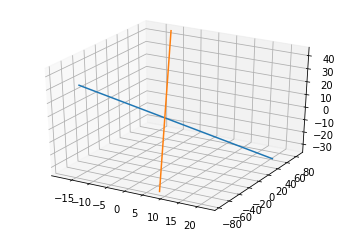
\includegraphics[width=\columnwidth]{figa.png}
    \caption{The plot of the lines}
    \end{figure}
    \item 
    The direction vectors $\vec{a}$ and $\vec{b}$ of the two lines are
    \begin{align}
        \vec{c}=\myvec{2\\2\\1}\\
        \vec{d}=\myvec{4\\1\\8}
    \end{align}
    Let $\theta$ be the angle between the vectors,
    \begin{align}
        cos\theta = \frac{\vec{c}^\top \vec{d}}{\norm{\vec{c}} {\norm{\vec{d}}}}
    \end{align}
    \begin{align}
        \vec{c}^\top\vec{d}&=\myvec{2&2&1}\myvec{4\\1\\8}\\
                           &=18
    \end{align}
    \begin{align}
        \norm{\vec{c}} &=3\\
        \norm{\vec{d}} &=9
    \end{align}
    \begin{align}
        \implies cos\theta & = \frac{18}{9\times 3}\\
          \theta &= \arccos\brak{\frac{2}{3}}\\
                 &= 48.189\degree
    \end{align}
   \begin{figure}[!ht]
   \centering
   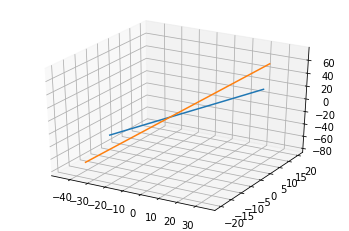
\includegraphics[width=\columnwidth]{figb.png}
   \caption{The plot the lines}
   \end{figure}
\end{enumerate}
    


\end{document}